% Options for packages loaded elsewhere
\PassOptionsToPackage{unicode}{hyperref}
\PassOptionsToPackage{hyphens}{url}
\PassOptionsToPackage{dvipsnames,svgnames,x11names}{xcolor}
%
\documentclass[
  letterpaper,
  DIV=11,
  numbers=noendperiod]{scrartcl}

\usepackage{amsmath,amssymb}
\usepackage{lmodern}
\usepackage{iftex}
\ifPDFTeX
  \usepackage[T1]{fontenc}
  \usepackage[utf8]{inputenc}
  \usepackage{textcomp} % provide euro and other symbols
\else % if luatex or xetex
  \usepackage{unicode-math}
  \defaultfontfeatures{Scale=MatchLowercase}
  \defaultfontfeatures[\rmfamily]{Ligatures=TeX,Scale=1}
\fi
% Use upquote if available, for straight quotes in verbatim environments
\IfFileExists{upquote.sty}{\usepackage{upquote}}{}
\IfFileExists{microtype.sty}{% use microtype if available
  \usepackage[]{microtype}
  \UseMicrotypeSet[protrusion]{basicmath} % disable protrusion for tt fonts
}{}
\makeatletter
\@ifundefined{KOMAClassName}{% if non-KOMA class
  \IfFileExists{parskip.sty}{%
    \usepackage{parskip}
  }{% else
    \setlength{\parindent}{0pt}
    \setlength{\parskip}{6pt plus 2pt minus 1pt}}
}{% if KOMA class
  \KOMAoptions{parskip=half}}
\makeatother
\usepackage{xcolor}
\setlength{\emergencystretch}{3em} % prevent overfull lines
\setcounter{secnumdepth}{-\maxdimen} % remove section numbering
% Make \paragraph and \subparagraph free-standing
\ifx\paragraph\undefined\else
  \let\oldparagraph\paragraph
  \renewcommand{\paragraph}[1]{\oldparagraph{#1}\mbox{}}
\fi
\ifx\subparagraph\undefined\else
  \let\oldsubparagraph\subparagraph
  \renewcommand{\subparagraph}[1]{\oldsubparagraph{#1}\mbox{}}
\fi


\providecommand{\tightlist}{%
  \setlength{\itemsep}{0pt}\setlength{\parskip}{0pt}}\usepackage{longtable,booktabs,array}
\usepackage{calc} % for calculating minipage widths
% Correct order of tables after \paragraph or \subparagraph
\usepackage{etoolbox}
\makeatletter
\patchcmd\longtable{\par}{\if@noskipsec\mbox{}\fi\par}{}{}
\makeatother
% Allow footnotes in longtable head/foot
\IfFileExists{footnotehyper.sty}{\usepackage{footnotehyper}}{\usepackage{footnote}}
\makesavenoteenv{longtable}
\usepackage{graphicx}
\makeatletter
\def\maxwidth{\ifdim\Gin@nat@width>\linewidth\linewidth\else\Gin@nat@width\fi}
\def\maxheight{\ifdim\Gin@nat@height>\textheight\textheight\else\Gin@nat@height\fi}
\makeatother
% Scale images if necessary, so that they will not overflow the page
% margins by default, and it is still possible to overwrite the defaults
% using explicit options in \includegraphics[width, height, ...]{}
\setkeys{Gin}{width=\maxwidth,height=\maxheight,keepaspectratio}
% Set default figure placement to htbp
\makeatletter
\def\fps@figure{htbp}
\makeatother
\newlength{\cslhangindent}
\setlength{\cslhangindent}{1.5em}
\newlength{\csllabelwidth}
\setlength{\csllabelwidth}{3em}
\newlength{\cslentryspacingunit} % times entry-spacing
\setlength{\cslentryspacingunit}{\parskip}
\newenvironment{CSLReferences}[2] % #1 hanging-ident, #2 entry spacing
 {% don't indent paragraphs
  \setlength{\parindent}{0pt}
  % turn on hanging indent if param 1 is 1
  \ifodd #1
  \let\oldpar\par
  \def\par{\hangindent=\cslhangindent\oldpar}
  \fi
  % set entry spacing
  \setlength{\parskip}{#2\cslentryspacingunit}
 }%
 {}
\usepackage{calc}
\newcommand{\CSLBlock}[1]{#1\hfill\break}
\newcommand{\CSLLeftMargin}[1]{\parbox[t]{\csllabelwidth}{#1}}
\newcommand{\CSLRightInline}[1]{\parbox[t]{\linewidth - \csllabelwidth}{#1}\break}
\newcommand{\CSLIndent}[1]{\hspace{\cslhangindent}#1}

\usepackage{booktabs}
\usepackage{longtable}
\usepackage{array}
\usepackage{multirow}
\usepackage{wrapfig}
\usepackage{float}
\usepackage{colortbl}
\usepackage{pdflscape}
\usepackage{tabu}
\usepackage{threeparttable}
\usepackage{threeparttablex}
\usepackage[normalem]{ulem}
\usepackage{makecell}
\usepackage{xcolor}
\KOMAoption{captions}{tableheading,figureheading}
\makeatletter
\makeatother
\makeatletter
\makeatother
\makeatletter
\@ifpackageloaded{caption}{}{\usepackage{caption}}
\AtBeginDocument{%
\ifdefined\contentsname
  \renewcommand*\contentsname{Table of contents}
\else
  \newcommand\contentsname{Table of contents}
\fi
\ifdefined\listfigurename
  \renewcommand*\listfigurename{List of Figures}
\else
  \newcommand\listfigurename{List of Figures}
\fi
\ifdefined\listtablename
  \renewcommand*\listtablename{List of Tables}
\else
  \newcommand\listtablename{List of Tables}
\fi
\ifdefined\figurename
  \renewcommand*\figurename{Figure}
\else
  \newcommand\figurename{Figure}
\fi
\ifdefined\tablename
  \renewcommand*\tablename{Table}
\else
  \newcommand\tablename{Table}
\fi
}
\@ifpackageloaded{float}{}{\usepackage{float}}
\floatstyle{ruled}
\@ifundefined{c@chapter}{\newfloat{codelisting}{h}{lop}}{\newfloat{codelisting}{h}{lop}[chapter]}
\floatname{codelisting}{Listing}
\newcommand*\listoflistings{\listof{codelisting}{List of Listings}}
\makeatother
\makeatletter
\@ifpackageloaded{caption}{}{\usepackage{caption}}
\@ifpackageloaded{subcaption}{}{\usepackage{subcaption}}
\makeatother
\makeatletter
\@ifpackageloaded{tcolorbox}{}{\usepackage[many]{tcolorbox}}
\makeatother
\makeatletter
\@ifundefined{shadecolor}{\definecolor{shadecolor}{rgb}{.97, .97, .97}}
\makeatother
\makeatletter
\makeatother
\ifLuaTeX
  \usepackage{selnolig}  % disable illegal ligatures
\fi
\IfFileExists{bookmark.sty}{\usepackage{bookmark}}{\usepackage{hyperref}}
\IfFileExists{xurl.sty}{\usepackage{xurl}}{} % add URL line breaks if available
\urlstyle{same} % disable monospaced font for URLs
\hypersetup{
  pdftitle={Death Registrations May Indicate a Discreptency Between Expected and Reported Data During the COVID-19 Pandemic},
  pdfauthor={Chloe Thierstein},
  colorlinks=true,
  linkcolor={blue},
  filecolor={Maroon},
  citecolor={Blue},
  urlcolor={Blue},
  pdfcreator={LaTeX via pandoc}}

\title{Death Registrations May Indicate a Discreptency Between Expected
and Reported Data During the COVID-19 Pandemic\thanks{Code and data are
available at:
https://github.com/cthierst/death\_registry\_analysis.git.}}
\usepackage{etoolbox}
\makeatletter
\providecommand{\subtitle}[1]{% add subtitle to \maketitle
  \apptocmd{\@title}{\par {\large #1 \par}}{}{}
}
\makeatother
\subtitle{An Analysis of Death Registrations from 2016-2020}
\author{Chloe Thierstein}
\date{3 February 2023}

\begin{document}
\maketitle
\begin{abstract}
The COVID-19 pandemic marked a significant shift in Canadian mortality
rates in the year 2020. Using death registry data from three civic
centres in the greater Toronto are from 2016 to 2020, we demonstrate
that even data from a considerably reliable source may become distorted
\end{abstract}
\ifdefined\Shaded\renewenvironment{Shaded}{\begin{tcolorbox}[interior hidden, boxrule=0pt, enhanced, borderline west={3pt}{0pt}{shadecolor}, breakable, frame hidden, sharp corners]}{\end{tcolorbox}}\fi

\hypertarget{introduction}{%
\section{1 Introduction}\label{introduction}}

Canadian death registry statistics offer a useful tool in helping better
our healthcare system as by monitoring trends in public health such as
infectious diseases, suicide, and unintentional injuries they help the
healthcare sector provide better services and resources, like screening
and prevention programs (Statistics Canada 2022b). However, maintaining
this data may not always be done accurately which could cause confusion
over our understanding of Canadian demography and health.

In this paper we look at death registry statistics from three civic
centres in the greater Toronto area, Etobicoke, Scarborough and North
York between 2016 and 2020. From this data, we find that the death
licenses provided by these centres during the first year of the COVID-19
pandemic (2020), are much lower than in previous years (Open Data
Toronto 2023). This is significant as Canada experienced an increase of
7.7\% in deaths in 2020 (Statistics Canada 2022a), and 5.2\% more deaths
than would typically be expected when taking into account Canada's aging
population (Statistics Canada 2021). We reason that this discrepancy in
expected data versus reported data could be the result of strain and
complications put onto record-keeping during this time similarly to what
was seen in early 2019 with long delays in the distribution of death,
birth and marriage certificates due to high online demand (Jeffords
2019). Future work could look specifically at how strains on data
reporting centres during the COVID-19 pandemic influenced data.

This paper will begin with an overview of its data management, source
and cleaning. Next we will briefly overview the drop off in trend from
previous years in death registrations to begin our discussion. Next we
will consider the relationship between death licenses provided at each
civic centre over the period of 2016 to 2020, to better understand how
the year 2020 differed from past years. Next, we discuss in more detail,
death licenses provided by each civic centre to determine a possible
cause for the uncharacteristic decline of death licenses in 2020. We
will then compare the mean number of deaths from each civic centre to
further gauge how these centres relate to rates of death registrations.
Finally, we will consider the limitations of the data, including biases.

\hypertarget{data}{%
\section{2 Data}\label{data}}

\hypertarget{data-management}{%
\subsection{2.1 Data Management}\label{data-management}}

This paper utilizes the R statistical programming language (R Core Team
2020), along with several packages. These packages are, tidyverse
(Wickham et al. 2019), janitor (Firke 2021), here (Müller 2020) and
dplyr (Wickham et al. 2022). The data being analyzed comes from Open
Data Toronto and it is imported using the opendatatoronto package
(Gelfand 2022). All figures have been created using ggplot2 (Wickham
2016) and the tables have been created with knitr (Xie 2023) and
kableExtra (Zhu 2021), packages. The color styles in the graphs were
created by using the RColorBrewer (Neuwirth 2022) package and any graph
combinations were made using the Patchwork (Pedersen 2022) package.

\hypertarget{data-source-and-cleaning}{%
\subsection{2.2 Data Source and
Cleaning}\label{data-source-and-cleaning}}

The data comes from death registrations which are entered into the
Registry Services Tracking System (RSTS) by Registry Services staff who
are located at three of the civic centres, Etobicoke, North York and
Scarborough (Open Data Toronto 2023). It's creation supports the Vital
Statistics Act, a Provincial legislation (Open Data Toronto 2023) which
involve the collection of deaths, marriages, stillbirths, and live
births (Statistics Canada 2022b). This data set is updated monthly (Open
Data Toronto 2023). The variables from this data set represent the civic
centres; ``Etobicoke'', ``North York'', and ``Scarborough'', number of
death licenses registered in the month, place of death; ``Outside City
Limits'' or ``Toronto'', and time period by month and year in which the
death was registered (Open Data Toronto 2023).

To properly analyze this data for the purposes of this paper certain
data was removed including, all data for the years 2011-2015 and
2021-2023. This was done to ensure that the data set being worked with
had sufficient and consistent data to draw from without being too broad
in scope. Additionally, rows from the civic centre variable labelled
``Toronto'' were removed as death registrations at this location were
especially low and its data input, sporadic. Finally, the variable for
place of death was not included in the analysis of this data as it was
not relevant to its narrative.

\hypertarget{data-analysis}{%
\subsection{2.3 Data Analysis}\label{data-analysis}}

The province of Ontario represents a large portion of deaths in Canada,
taking on an estimated 37\% of Canadian mortality from 2016-2020
(Statistics Canada n.d.). It is also estimated that on average, that
just over 100 thousand people have died each year in Ontario between
2016 and 2020 (Statistics Canada n.d.). We may suggest then, that
Toronto makes up a large portion of this mortality rate, as it makes up
approximately 44\% of the Ontarian population (Statistics Canada n.d.).
Additionally, Canada has an aging population, meaning that it's
mortality rate is expected to rise every year although it rose
exponentially due to the COVID-19 pandemic (Statistics Canada 2022a).
Therefore, we may suspect that the COVID-19 pandemic would increase the
mortality rate significantly in Toronto as Canada saw an increase of
7.7\% in deaths in 2020 (Statistics Canada 2022a).

\begin{figure}

\caption{\label{fig-1}Death Licenses Provided by All Civic Centres
Yearly From 2016-2020}

{\centering \includegraphics{paper_files/figure-pdf/fig-1-1.pdf}

}

\end{figure}

When looking at Figure~\ref{fig-1}, however, we can see that from 2016
to 2018 to there was an increase in death licenses registered, as
expected, followed by a slight drop in 2019. This drop in 2019 may be
indicative of a backlog from Ontario's Vital Statistics in early 2019
which was cited as having delays of over three months, waiting for
death, birth and marriage certificates (Jeffords 2019). What is most
important in Figure~\ref{fig-1} is that when looking at the ``2020'' bar
in Figure~\ref{fig-1}, we can see that the death licenses registered
drops significantly in comparison to any of the previous 4 months.

\begin{figure}

\caption{\label{fig-2}Death Licenses Provided by Month from 2016-2020 at
Three Toronto Civic Centres}

{\centering 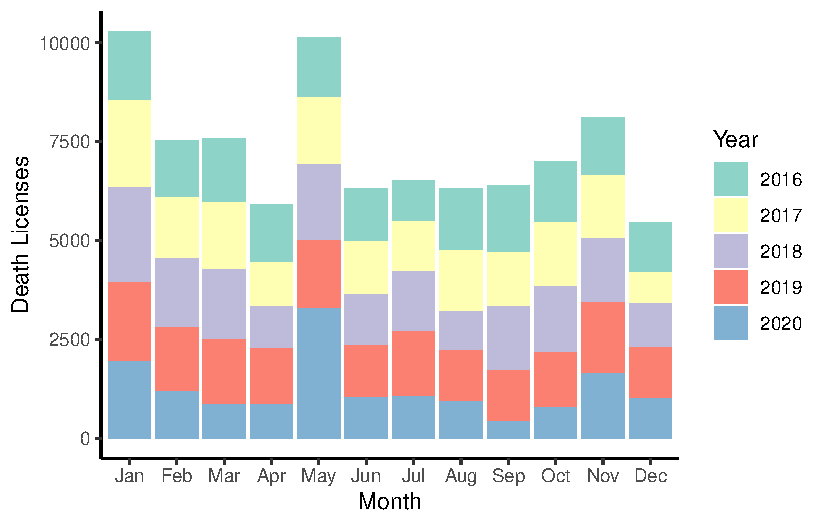
\includegraphics{paper_files/figure-pdf/fig-2-1.pdf}

}

\end{figure}

when looking at Figure~\ref{fig-2} we can see - death licenses provided
by month and year from all three civic centres - highlights the spike in
death licenses provided in May - this may indicate a spike in deaths
near the beginning of COVID-19 pandemic, - \textasciitilde need to find
source to make this make sense\textasciitilde{}

\begin{figure}

\caption{\label{fig-3}Death Licenses Provided by Each Civic Centre
Yearly and Monthly from 2016-2020}

{\centering 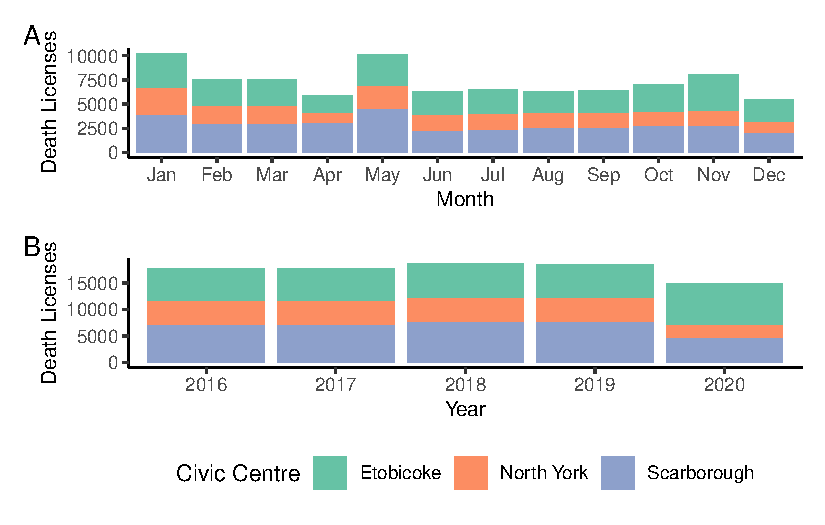
\includegraphics{paper_files/figure-pdf/fig-3-1.pdf}

}

\end{figure}

Looking briefly at Figure~\ref{fig-3} we can see a surprising drop in
death licenses provided in 2020. \#\#\#\#\#\# this is surprising as
death rates are said to have increased during the pandemic, yet there is
a signficant decline \#\#\#\#\#\# why? explain\ldots{}

\hypertarget{tbl-1}{}
\begin{table}
\caption{\label{tbl-1}Average Number of Deaths Per Month from 2016-2020 at Etobicoke Centre }\tabularnewline

\centering
\begin{tabular}{lrrrrr}
\toprule
\multicolumn{1}{c}{ } & \multicolumn{5}{c}{Average Number of Deaths} \\
\cmidrule(l{3pt}r{3pt}){2-6}
Month & 2016 & 2017 & 2018 & 2019 & 2020\\
\midrule
Jan & 342 & 360 & 372 & 346 & 358\\
Feb & 264 & 276 & 275 & 259 & 250\\
Mar & 275 & 281 & 285 & 269 & 237\\
Apr & 236 & 209 & 211 & 237 & 273\\
May & 315 & 320 & 329 & 320 & 403\\
Jun & 236 & 238 & 235 & 253 & 196\\
Jul & 223 & 250 & 263 & 275 & 235\\
Aug & 241 & 239 & 211 & 230 & 210\\
Sep & 248 & 225 & 251 & 236 & 185\\
Oct & 281 & 275 & 275 & 278 & 226\\
Nov & 348 & 351 & 340 & 356 & 280\\
Dec & 229 & 209 & 233 & 228 & 217\\
\bottomrule
\end{tabular}
\end{table}

\hypertarget{tbl-2}{}
\begin{table}
\caption{\label{tbl-2}Average Number of Deaths Per Month from 2016-2020 at Scarborough Centre }\tabularnewline

\centering
\begin{tabular}{lrrrrr}
\toprule
\multicolumn{1}{c}{ } & \multicolumn{5}{c}{Average Number of Deaths} \\
\cmidrule(l{3pt}r{3pt}){2-6}
Month & 2016 & 2017 & 2018 & 2019 & 2020\\
\midrule
Jan & 350 & 366 & 376 & 371 & 359\\
Feb & 266 & 269 & 272 & 289 & 262\\
Mar & 275 & 281 & 273 & 284 & 244\\
Apr & 273 & 262 & 261 & 268 & 299\\
May & 382 & 396 & 409 & 382 & 419\\
Jun & 214 & 214 & 201 & 206 & 223\\
Jul & 253 & 248 & 263 & 253 & 274\\
Aug & 275 & 279 & 252 & 271 & 288\\
Sep & 252 & 243 & 244 & 236 & 195\\
Oct & 256 & 264 & 258 & 244 & 226\\
Nov & 246 & 256 & 265 & 261 & 301\\
Dec & 214 & 184 & 199 & 203 & 272\\
\bottomrule
\end{tabular}
\end{table}

\hypertarget{tbl-3}{}
\begin{table}
\caption{\label{tbl-3}Average Number of Deaths Per Month from 2016-2020 at North York Centre }\tabularnewline

\centering
\begin{tabular}{lrrrrr}
\toprule
\multicolumn{1}{c}{ } & \multicolumn{5}{c}{Average Number of Deaths} \\
\cmidrule(l{3pt}r{3pt}){2-6}
Month & 2016 & 2017 & 2018 & 2019 & 2020\\
\midrule
Jan & 291 & 323 & 330 & 303 & 293\\
Feb & 210 & 214 & 236 & 222 & 193\\
Mar & 224 & 221 & 235 & 225 & 182\\
Apr & 184 & 164 & 155 & 180 & 189\\
May & 246 & 250 & 259 & 268 & 372\\
Jun & 194 & 193 & 199 & 179 & 180\\
Jul & 176 & 186 & 194 & 211 & 209\\
Aug & 199 & 195 & 165 & 172 & 186\\
Sep & 198 & 181 & 194 & 170 & 135\\
Oct & 183 & 192 & 205 & 176 & 160\\
Nov & 194 & 200 & 204 & 220 & 233\\
Dec & 165 & 139 & 151 & 184 & 189\\
\bottomrule
\end{tabular}
\end{table}

\clearpage

\hypertarget{references}{%
\section*{References}\label{references}}
\addcontentsline{toc}{section}{References}

\hypertarget{refs}{}
\begin{CSLReferences}{1}{0}
\leavevmode\vadjust pre{\hypertarget{ref-citejanitor}{}}%
Firke, Sam. 2021. \emph{Janitor: Simple Tools for Examining and Cleaning
Dirty Data}. \url{https://CRAN.R-project.org/package=janitor}.

\leavevmode\vadjust pre{\hypertarget{ref-citeopendatatoronto}{}}%
Gelfand, Sharla. 2022. \emph{Opendatatoronto: Access the City of Toronto
Open Data Portal}.
\url{https://CRAN.R-project.org/package=opendatatoronto}.

\leavevmode\vadjust pre{\hypertarget{ref-citectvnews}{}}%
Jeffords, Shawn. 2019. {``Delays in Birth, Death, Marriage Certificates
Caused by High Demand, Online Issues.''} CTV News Windsor.
\url{https://windsor.ctvnews.ca/delays-in-birth-death-marriage-certificates-caused-by-high-demand-online-issues-1.4305301}.

\leavevmode\vadjust pre{\hypertarget{ref-citehere}{}}%
Müller, Kirill. 2020. \emph{Here: A Simpler Way to Find Your Files}.
\url{https://CRAN.R-project.org/package=here}.

\leavevmode\vadjust pre{\hypertarget{ref-citercolorbrewer}{}}%
Neuwirth, Erich. 2022. \emph{RColorBrewer: ColorBrewer Palettes}.
\url{https://CRAN.R-project.org/package=RColorBrewer}.

\leavevmode\vadjust pre{\hypertarget{ref-citeopendatatoronto2}{}}%
Open Data Toronto. 2023. {``Death Registry Statistics.''} City of
Toronto Open Data Portal.
\url{https://open.toronto.ca/dataset/death-registry-statistics/}.

\leavevmode\vadjust pre{\hypertarget{ref-citepatchwork}{}}%
Pedersen, Thomas Lin. 2022. \emph{Patchwork: The Composer of Plots}.
\url{https://CRAN.R-project.org/package=patchwork}.

\leavevmode\vadjust pre{\hypertarget{ref-citeR}{}}%
R Core Team. 2020. \emph{R: A Language and Environment for Statistical
Computing}. Vienna, Austria: R Foundation for Statistical Computing.
\url{https://www.R-project.org/}.

\leavevmode\vadjust pre{\hypertarget{ref-citestatscan1}{}}%
Statistics Canada. n.d. {``Table 17-10-0008-01 Estimates of the
Components of Demographic Growth, Annual.''}
\url{https://doi.org/10.25318/1710000801-eng}.

\leavevmode\vadjust pre{\hypertarget{ref-citestatscan2}{}}%
---------. n.d. {``Table 17-10-0135-01 Population Estimates, July 1, by
Census Metropolitan Area and Census Agglomeration, 2016 Boundaries.''}
\url{https://doi.org/10.25318/1710013501-eng}.

\leavevmode\vadjust pre{\hypertarget{ref-citestatscan5}{}}%
---------. 2021. {``Provisional Death Counts and Excess Mortality,
January 2020 to August 2021.''}
\url{https://www150.statcan.gc.ca/n1/daily-quotidien/211108/dq211108a-eng.htm}.

\leavevmode\vadjust pre{\hypertarget{ref-citestatscan4}{}}%
---------. 2022a. {``Deaths, 2020.''}
\url{https://www150.statcan.gc.ca/n1/daily-quotidien/220124/dq220124a-eng.htm}.

\leavevmode\vadjust pre{\hypertarget{ref-citestatscan3}{}}%
---------. 2022b. {``Frequently Asked Questions on Vital Statistics.''}
\url{https://www.statcan.gc.ca/en/about/relevant/vscc/faq}.

\leavevmode\vadjust pre{\hypertarget{ref-citeggplot2}{}}%
Wickham, Hadley. 2016. \emph{Ggplot2: Elegant Graphics for Data
Analysis}. Springer-Verlag New York.
\url{https://ggplot2.tidyverse.org}.

\leavevmode\vadjust pre{\hypertarget{ref-citetidyverse}{}}%
Wickham, Hadley, Mara Averick, Jennifer Bryan, Winston Chang, Lucy
D'Agostino McGowan, Romain François, Garrett Grolemund, et al. 2019.
{``Welcome to the {tidyverse}.''} \emph{Journal of Open Source Software}
4 (43): 1686. \url{https://doi.org/10.21105/joss.01686}.

\leavevmode\vadjust pre{\hypertarget{ref-citedplyr}{}}%
Wickham, Hadley, Romain François, Lionel Henry, and Kirill Müller. 2022.
\emph{Dplyr: A Grammar of Data Manipulation}.
\url{https://CRAN.R-project.org/package=dplyr}.

\leavevmode\vadjust pre{\hypertarget{ref-citeknitr}{}}%
Xie, Yihui. 2023. \emph{Knitr: A General-Purpose Package for Dynamic
Report Generation in r}. \url{https://yihui.org/knitr/}.

\leavevmode\vadjust pre{\hypertarget{ref-citekablextra}{}}%
Zhu, Hao. 2021. \emph{kableExtra: Construct Complex Table with 'Kable'
and Pipe Syntax}. \url{https://CRAN.R-project.org/package=kableExtra}.

\end{CSLReferences}



\end{document}
